% =====================================================================
% sections/results.tex
% Results and analyses section -- input by report.tex.
%
% Word budget: ~1300 words (results + analyses combined; counted toward the
% 3000-word limit). Spec: short subsections are normal; resist padding.
%
% Order builds to the two main points (MP1 = assimilation verdict;
% MP2 = Dev only paradox):
%   1. Substrate-level sanity check (HP works at the network level)
%   2. Four-condition replication (which condition wins on fitness)
%   3. Search replication (early-progress read; Williams's qualitative claim)
%   4. Behavioural trajectories (qualitative differences across conditions)
%   5. Viable-range diagnostics (mechanistic bridge: HP-off collapse)
%   6. Frozen-HP test (MP1 lands here)
%   7. Search dynamics (the larger adaptive system; closes the section)
%
% Filenames assume figs/ contents per todo.md and README. Verify before
% compiling: substrate_check.pdf, replication_fitness_curves.pdf,
% replication_final_box.pdf, behavioural_trajectories.pdf,
% viable_range_compact.pdf, frozen_hp_scatter.pdf, frozen_hp_drop.pdf,
% search_dynamics_population.pdf.
% =====================================================================

\section{Results and analyses}
\label{sec:results}

\subsection{Substrate-level sanity check}
\label{sec:results:substrate}

Before evolving controllers, the homeostatic plasticity rule was verified on
isolated networks. One hundred random five-node CTRNNs were instantiated with
parameters sampled from the evolution ranges
(Table~\ref{tab:param-ranges}). Each was run for $220$ timesteps with $I = 0$ and
HP disabled to establish a baseline, then for $6000$ timesteps with HP
active, and finally for a further $220$ timesteps with HP disabled to test
whether the homeostatic effect persisted. The fraction of firing-rate samples
falling outside $[H_L, H_U]$ was $0.861$ before HP, $0.532$ during HP, and
$0.594$ after HP was switched off (Figure~\ref{fig:substrate}). HP halves the
out-of-range fraction during its operation and the improvement partly persists
once HP is disabled, confirming that the rule reshapes the network's parameters
rather than masking saturation dynamically. The residual gap between during-HP
and after-HP samples is the same kind of HP-dependent operation the frozen-HP
test (Section~\ref{sec:results:frozenhp}) probes in evolved networks.

\begin{figure}[t]
  \centering
  % 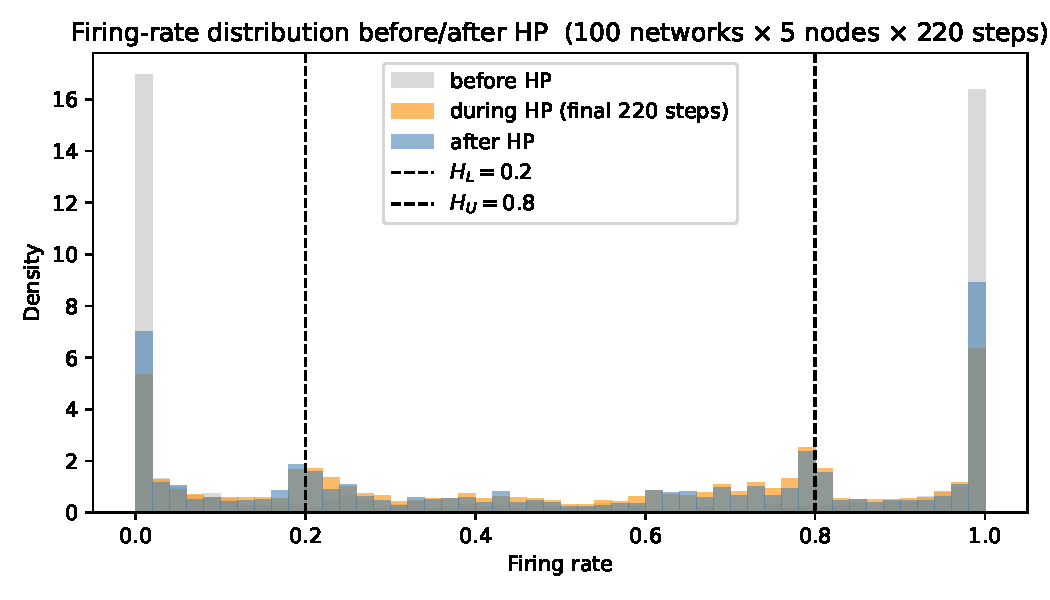
\includegraphics[width=0.7\linewidth]{figs/substrate_check.pdf}
  \caption{Substrate-level sanity check. Firing-rate distributions of
  100 random CTRNNs before HP, during HP, and after HP was switched off.
  Dashed lines mark $H_L = 0.2$ and $H_U = 0.8$.}
  \label{fig:substrate}
\end{figure}

\subsection{Replicating Williams's evolvability ordering}
\label{sec:results:replication}

Ten evolutionary runs per condition produced the fitness curves and final-fitness
distribution shown in Figure~\ref{fig:replication}. Mean best-of-generation
fitness across the ten runs is plotted with a $\pm 1$ standard-deviation band
and individual runs faintly overlaid; the final-fitness panel shows all ten
run-final values as points.

Final-fitness means (SDs in parentheses) are: \emph{No HP} $0.674$ ($0.096$),
\emph{Dev only} $0.838$ ($0.059$), \emph{Behaviour only} $0.709$ ($0.097$),
\emph{Both} $0.675$ ($0.077$). A Kruskal--Wallis test across the four
conditions gives $H = 17.71$, $p = 0.0005$. Pairwise Mann--Whitney $U$ tests
with Bonferroni correction (six pairs) place \emph{Dev only} significantly above
each of the other three conditions: vs.\ \emph{No HP} $p_{\text{bonf}} = 0.0035$,
vs.\ \emph{Behaviour only} $p_{\text{bonf}} = 0.0217$, vs.\ \emph{Both}
$p_{\text{bonf}} = 0.0035$. \emph{No HP}, \emph{Behaviour only} and \emph{Both}
are mutually indistinguishable (all pairwise $p_{\text{bonf}} = 1.000$).

The qualitative ordering reproduces Williams's: a developmental HP phase before
evaluation produces the best evolved fitness. The departure from Williams is
that \emph{Behaviour only} and \emph{Both} are not statistically worse than
\emph{No HP} in our data, whereas Williams reports them as worse; the
implications of this divergence are taken up in
Section~\ref{sec:discussion}.

\begin{figure}[t]
  \centering
  % \includegraphics[width=\linewidth]{figs/replication_fitness_curves.pdf}\par\medskip
  % \includegraphics[width=0.7\linewidth]{figs/replication_final_box.pdf}
  \caption{Four-condition replication ($n = 10$ runs per condition,
  $200$ generations). Top: best-of-generation fitness, mean across runs with
  $\pm 1$~SD band and individual runs faint. Bottom: final-generation best
  fitness, all ten runs as points.}
  \label{fig:replication}
\end{figure}

\subsection{Search replication: early progress and run consistency}
\label{sec:results:searchreplication}

Williams reports two qualitative search-level observations about plastic
networks: faster early progress and greater run-to-run consistency. Both are
visible in Figure~\ref{fig:replication}. \emph{Dev only} reaches a clearly
higher mean fitness within the first ten generations than any of the other
three conditions and remains the most consistent across runs (the smallest
final-fitness SD, $0.059$). The other three conditions improve gradually across
all $200$ generations and show comparable run-to-run spread. The pattern that
\emph{plastic} networks have an early advantage over non-plastic networks
\emph{when the plasticity acts before evaluation} is reproduced; the further
claim, that online HP also accelerates early progress, is not, and tracks the
non-significance of the online-HP conditions in the final-fitness comparison.

\subsection{Behavioural trajectories}
\label{sec:results:trajectories}

To see what the evolved controllers actually \emph{do}, the best individual
from each condition was replayed across three shared-seed trials with
per-timestep recording of agent position, shape position, and neural firing
rates (Figure~\ref{fig:trajectories}). Firing-rate cells are coloured by
viable-range state: blue below $H_L$, cream within $[H_L, H_U]$, red above
$H_U$. All four representative individuals track the falling shapes
competently; the differences are in the underlying neural activity.

The \emph{No HP} individual operates with all neurons saturated, mostly red
or blue, for nearly the whole trial: each neuron settles on one rail and stays
there. The \emph{Dev only} individual, despite running with HP frozen during the
trial, shows pronounced banding --- neurons alternate between above-range and
below-range and rarely remain saturated for long. The \emph{Behaviour only}
individual operates largely within the viable range, with one sensor neuron
showing the same banding pattern seen in \emph{Dev only}; \emph{Both} shows
broader bands and more in-range time than \emph{No HP} or \emph{Dev only}.

\begin{figure}[t]
  \centering
  % \includegraphics[width=\linewidth]{figs/behavioural_trajectories.pdf}
  \caption{Behavioural trajectories for the best individual per condition,
  three shared-seed trials each. Top of each panel: agent and shape
  $x$-positions over time. Bottom: five-neuron firing-rate heatmap; blue
  $z < H_L$, cream $z \in [H_L, H_U]$, red $z > H_U$.}
  \label{fig:trajectories}
\end{figure}

\subsection{Viable-range diagnostics across evolution}
\label{sec:results:viablerange}

The qualitative differences in Section~\ref{sec:results:trajectories} are
quantified at population level by two per-neuron metrics computed at sampled
generations: $\mathrm{frac}_V$, the fraction of timesteps the firing rate lies
in $[H_L, H_U]$; and the \emph{entry--exit rate}, the number of transitions
per $1000$ timesteps between in-range and out-of-range states. Each metric is
computed in two modes: with HP active (the training mode) and with HP frozen
(adiabatic elimination).

Final-generation means across runs and neurons
(Figure~\ref{fig:viablerange}) show that with HP active, all three HP conditions
achieve $\mathrm{frac}_V$ between $0.43$ and $0.45$, well above the \emph{No HP}
baseline of $0.19$. With HP frozen, \emph{Dev only} and \emph{Behaviour only}
collapse to $\mathrm{frac}_V \approx 0.08$, at or below the \emph{No HP}
baseline; \emph{Both} retains slightly more activity in range ($0.16$). The
entry--exit rate distinguishes the developmental conditions from \emph{No HP}:
\emph{Dev only} in training mode shows $9.55$ transitions per $1000$ steps
versus \emph{No HP}'s $1.49$ (the banding seen in
Figure~\ref{fig:trajectories}); when HP is frozen, \emph{Dev only}'s rate falls
to $0.04$. The pattern is the same in all three HP conditions: viable-range
operation is held in place by HP and collapses when HP is removed.

\begin{figure}[t]
  \centering
  % \includegraphics[width=\linewidth]{figs/viable_range_compact.pdf}
  \caption{Per-neuron viable-range diagnostics, mean across runs and neurons
  at the final generation. Left: $\mathrm{frac}_V$ with HP active and with
  HP frozen. Right: final-generation entry--exit rate per $1000$ timesteps,
  HP active.}
  \label{fig:viablerange}
\end{figure}

\subsection{Frozen-HP test: has assimilation occurred?}
\label{sec:results:frozenhp}

The central extension is the frozen-HP test, which asks whether the behaviour
evolved under HP persists once HP is removed. Each evolved individual was
re-evaluated twice: once with HP active (the training condition) and once with
HP frozen by adiabatic elimination after a settling window. Within-individual
measurement noise was estimated by re-evaluating each individual $20$ times with
different shape-sequence seeds and HP active; frozen-HP fitness drops are
reported in units of this within-individual SD.

The control conditions confirm the test isolates HP-dependence rather than
measurement noise: \emph{No HP} individuals show drops within $\pm 1$ SD
(no HP was active in their training, so freezing should have no effect), and
this is what is observed. The HP conditions show a clear departure from this
baseline (Figure~\ref{fig:frozenhp}). \emph{Dev only} individuals drop by
$5.6$--$28.8$ SD, with $5/10$ collapsing to zero fitness when evaluated from
the genotype without development. \emph{Behaviour only} drops span
$0.2$--$17.4$ SD with $3/10$ complete or near-complete collapses. \emph{Both}
shows a similar bimodal pattern: $3/10$ complete collapses ($11.6$--$16.5$ SD),
the remainder showing moderate drops.

The headline finding is that no HP condition shows the small drops that genetic
assimilation would predict. The behaviour is HP-dependent across all three HP
conditions: in a substantial fraction of individuals (between $3/10$ and $5/10$
depending on condition) HP is not merely beneficial but constitutive ---
removing it collapses the behaviour entirely.

\begin{figure}[t]
  \centering
  % \includegraphics[width=\linewidth]{figs/frozen_hp_scatter.pdf}\par\medskip
  % \includegraphics[width=0.7\linewidth]{figs/frozen_hp_drop.pdf}
  \caption{Frozen-HP test. Top: HP-active fitness against frozen-HP fitness for
  each of the $40$ final-generation best individuals, by condition; the dashed
  line $y = x$ marks zero drop. Bottom: drop magnitude per individual in units
  of the within-individual measurement-noise SD.}
  \label{fig:frozenhp}
\end{figure}

\subsection{Search dynamics of the larger adaptive system}
\label{sec:results:searchdynamics}

The analyses above examine the evolved controller. The fourth analysis examines
the search itself. Per-generation population best, mean, and fitness spread were
computed from the full saved population fitness arrays
(Figure~\ref{fig:searchdynamics}). Three observations: first, all four
conditions converge on a similar timescale --- the population fitness spread
collapses to near zero by roughly generations $10$ to $20$ in every condition.
Second, fitness continues to improve after the spread collapses, consistent
with refinement within a converged gene pool rather than a stalled search.
Third, and most importantly, the conditions differ in \emph{where} they
converge, not whether or how fast: \emph{Dev only} converges to a markedly
higher final population mean than the others. HP does not change the rate or
character of convergence; it changes the basin the search settles into. The
discussion (Section~\ref{sec:discussion}) takes this up as the search-dynamics
read on Williams's result.

\begin{figure}[t]
  \centering
  % \includegraphics[width=\linewidth]{figs/search_dynamics_population.pdf}
  \caption{Population-level search dynamics, one panel per condition. Solid
  line: population best fitness per generation. Dashed line: population mean.
  Shaded band: population fitness SD (a diversity proxy).}
  \label{fig:searchdynamics}
\end{figure}
